\documentclass[12pt,english]{article}
\usepackage[T1]{fontenc}
\usepackage[latin9]{inputenc}
\usepackage{amsmath}
\usepackage{graphicx}

\makeatletter
\usepackage[letterpaper,body={6.5in,9in}, head=34pt, foot=70pt]{geometry}
\usepackage{fancyhdr}

\pdfpagewidth 8.5in
\pdfpageheight 11in

\pagestyle{fancy}
\headheight 35pt

\rhead{Fall 2021}
\chead{}
\lhead{MATH 3700 Operations Research}
\renewcommand{\footrulewidth}{0.4pt}
\rfoot{\thepage}
\cfoot{}
\lfoot{Wentworth Institute of Technology}

\usepackage{multicol}

\makeatother

\usepackage{babel}
\begin{document}
\textbf{Homework Assignment 2}\vspace{0.4cm}

\textbf{Due: }Monday, October 4, 2021 in GS.\vspace{0.6cm}

\textbf{Name: Sunny Lee\underline{\hspace{12cm}}\vspace{0.4cm}}
\begin{enumerate}
\item A furniture manufacturer makes two types of furniture: chairs and sofas. The production of the sofas and chairs requires three operations: carpentry, finishing, and upholstery. Manufacturing a chair requires 3 hours of carpentry, 9 hours of finishing, and 2 hours of upholstery. Manufacturing a sofa requires 2 hours of carpentry, 4 hours of finishing, and 10 hours of upholstery. The factory has allocated at most 66 labor hours for carpentry, 180 labor hours for finishing, and 200 labor hours for upholstery. The profit per chair is \$90 and the profit per sofa is \$75. \\

    The manufacturer wants to know how many chairs and how many sofas should be produced each day to maximize the profit. Formulate a linear programming (LP)problem you would use to find a solution.

\begin{gather*}
    max \quad z = 90x_1 + 75 x_2\\
    \text{subject to }\\
    3x_1 + 2x_2 \leq 66\\
    9x_1+4x_2 \leq 180\\
    2x_1 + 10x_2 \leq 200
\end{gather*}

\item Solve the LP problem you formulated in part 1, by using the simplex method (tableau method) and writing down the corresponding tableaux as done in class. Write down the row reductions you've used to move from one tableau to the next one. State your optimal solution (if any).
\[
\begin{array}{c | cccccc | c}
    & x_1 & x_2 & s_1 & s_2 & s_3 & z & \\
    s_1 & 3 &2 &1& 0& 0& 0& 66\\
    s_2 &9 &4 &0& 1 &0 &0& 180 \\
    s_3& 2& 10& 0& 0& 1& 0& 200\\
    &-90 &-75& 0& 0& 0& 1& 0 
\end{array}
\]

To get to the first tableau: $1/9R_1, -3R_2 + R_1, -2R_2+R_3, 90R_2+R_4$\\
To get to the second tableau: $3/2R_1, -4/9R_1 + R_2, -9/82R_1+R_3, 35R_1+R_4$\\
Finally:$3R_2, 1/2R_2+R_1, 242/1476R_2+R_3, 15/2R_2+R_4$ and we end up with 
2475 as our maximum. 
\item
    \begin{itemize}
        \item For this question you must have MS Excel installed in your computer and be able to use the \textit{Solver} add-in. If you have any trouble check again the handout on how to use Excel's \textit{Solver} for linear programming (material is in Brightspace).
        \item Set up an Excel sheet with the information of this LP problem.
        \item Use Excel \textit{Solver} to compute the solution to this problem.
        \item Include in your report a screenshot of the Excel sheet you used to find a solution.
        \item Compare the solution of the Excel Solver to the one you've gotten using the simplex. Are they the same?
    \end{itemize}
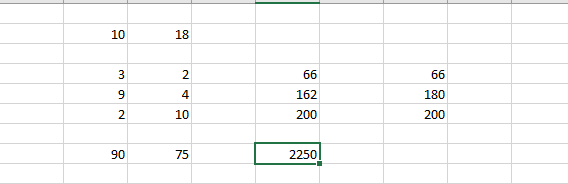
\includegraphics{number3.png}\\
Using the simplex method in excel, we find that the optimal solutions differ. 
\end{enumerate}

\end{document}